\section{Energy storage research for LV application}
\label{ch-literature:sec:energy-storage}

The challenge for DNOs to manage their distribution networks is caused by the DER's and LCT's difficult predictability, their volatile nature, and the weakness of the network into which they are deployed.
If left unmanaged, voltage fluctuations caused for example by PV systems \cite{Woyte2006, Bravo2015} or capacity shortages due to additional loads like EVs \cite{Mohd2008a, Koureoumpezis2010} will threaten the power system's stability.
Improved network management methods that are summarised under the term ``smart grid'' have thus become increasingly popular to counteract the negative impact from DERs and LCTs \cite{Panteli2015}.
However, when deferring the reinforcement or retrofitting of network assets to construct such a smart grid, deployment of BESS can provide a significant contribution to the integration of DERs and LCTs.
For instance, Grillo et al. in \cite{Grillo2012} showed how probabilistic price driven storage control successfully supports renewable integration.
Their simulated and validated BESS model provides arbitrage functions through generation shifting and was able to achieve a daily gain of more than \texteuro130.
But such an immediate financial benefit can only be achieved when their dynamic pricing is implemented and the repetitive discharge to 20\% does not shorten the BESS lifetime.
Focusing on grid support instead, Rowe et al. in \cite{Rowe2014a} showed how a BESS schedule can maximise the peak reduction capability in order to free system resources.
Since their BESS schedules were based on sometimes unreliable demand forecasts, they had to implement filtering operations to vary the forecast's peak magnitude, peak width and peak shape.
This filtering maximised the resulting peak reduction performance to a median peak reduction between 5kW to 7kW (instead of 0kW when no forecast filtering was implemented).
Similarly Hosseina et al. in \cite{Hosseina2016a} also used residential load forecasts to schedule BESS operation in order to level demand by shaving peak load.
Their BESS was installed in the medium voltage distribution network since their redox flow-battery was significantly larger than the lithium-ion battery that was used by Rowe et al. (i.e. 34MWh instead of 25kWh).
Apart from the difference in scale, both pieces of research used residential load forecasts only whilst Li et al. solved a stochastic unit commitment and economic dispatch problem to maximise renewable integration in \cite{Li2016}.
Unlike traditionally scheduled BESS operation, Li et al. also simulated real-time operation but assumed perfect demand and pricing knowledge at the time of operation.
As a result they achieved a financial gain of more than \$34000, but did not guarantee the BESS impact on the underlying power distribution network.

Over the past decade electricity DNOs and supplier branches from the Big Six (i.e. the UK's six major energy suppliers) begun trialling of BESS across their distribution network to better their understanding and potential contribution.
This was done since the BESS benefits had only been estimated and not thoroughly studied through field trials.
Showcase examples from some DNOs include:
\begin{itemize}
	\item Scottish and Southern Electricity Networks (SSEN) in \cite{NTVV2016} where BESSs were deployed in Bracknell distribution networks to uphold voltage stability and power quality;
	\item EDF Energy Networks in \cite{Wade2010} where BESS was installed in the 11kV distribution network for power flow management and to validate and improve system models;
	\item UK Power Networks (UKPN) in \cite{Lyons2015a} where BESS was installed to shave load peaks and level supply volatility from an adjacent wind farm;
\end{itemize}
and showcase examples from some of the energy suppliers include:
\begin{itemize}
	\item E.ON UK in \cite{EON2017} where a 5MWh BESS was colocated with a combined heat and power plant to stabilise its energy supply; and
	\item Scottish Power in \cite{ScottishPower2016} where 1MWh of distributed batteries were installed in households to support grid operation through flexible tariffs.
\end{itemize}
Nonetheless, from lessons learnt and aiming to meet statutory and physical restrictions under the future load changes, voltage control and the power flow problem have been identified as the two key challenges for DNOs \cite{Ferreira2013a, Shi2015}.

\subsection{Voltage control}
\label{ch-literature:subsec:voltage-control}

LV distribution networks in the UK operate at 230V Phase to Neutral (P2N) or 400V Phase to Phase (P2P) and have a statutory tolerance band of $\text{+10\% and -6\%}$.
But these voltages can deviate significantly due to the varying load on the network.
Although todays deviations may infrequently exceed high-voltage or low-voltage thresholds, conduction losses and imperfect network conditions result in a lower overall system efficiency.
Traditionally, On-Line Tap Changers (OLTCs) are used to raise and lower voltages across the entire LV distribution network in order to counteract voltage deviations \cite{Sun2009}.
However, such a hierarchical voltage control with OLTCs has its limited applicability, especially in cases where the voltage deviation significantly differs along individual branches of a feeding network \cite{Zangs2016}.
More specifically, if voltages diverge along different branches or different phases of a feeder due to asymmetric loads then the adjustment of transformer taps will lead to high or low voltage violations regardless of the tap change direction.
Installing a BESS at a strategic location (i.e. closer to the regions where voltage deviation takes place) and controlling the device to best suit the network's requirements is generally more applicable and commercially the more viable alternative \cite{Liserre2010}.

As stated by Wade et al. \cite{Wade2009}, allocation of the BESS's limited storage capacity so it can solve the voltage problem most effectively is still a sophisticated challenge.
Nonetheless, by installing a 200kWh unit that is rated at 600kW in a project that was carried out with \textit{EDF Energy}, they showed the potential of BESS in a network to provide targeted voltage support \cite{Wade2010}.
Their results for a 0.4MWh BESS achieved a reduced voltage variation by 2.4\% which resulted in a complete elimination of any ``out-of-limit'' voltage events, and a 70.96\% reduction of all network events (including power events) over the annual simulation period.
A demonstration project in Germany that was titled ``More Microgrids'' used four 180kWh batteries and demonstrated how both voltage stability as well as grid independence could be improved \cite{Overbeeke2010}.
In this ``More Microgrids'' project a collection of holiday homes were fitted with a distributed PV system that is capable of generating a peak power of 315kW, and BESS was used to maximise the utility from this generation.
However, due to the relatively small size of the network, due to the different behavioural patterns of holiday home occupants, and due to the different means of connecting customers to the German three-phase network, voltage deviation and phase unbalance issues were not as big as a concern as they are for UK distribution feeders.
An equally sized German project entitled ``GROWDERS'' also used multiple BESS in the LV network, but instead of focusing at grid independent network operation, they mainly contributed to frequency and thermal constraints as well as voltage stability \cite{GROWDERS2011}.

BESS that are sized between 100kWh to 200kWh (as those in the aforementioned projects \cite{Wade2010, Wade2009, Overbeeke2010, GROWDERS2011}) can easily address network issues, especially even when operating in a grid independent or ``islanded'' mode.
Results from these early field trials show how BESS store the excess renewable power for usage during later times.
But neither high nor low voltage events could be omitted once capacity limits were reached.
An oversized BESS would be less likely to meet its operating limits, but the associated cost makes this oversizing unfeasible.
Findings therefore indicate that not only the sizing, but also the BESS control method is of significant importance.
Nonetheless, continuous voltage violations that require strong voltage support have not yet been encountered in any of these projects, and instead occasional violations accumulating to less than an average of 1.1 minutes (instead of 2.3 minutes) per day are the norm \cite{Sugihara2013}.
Also, the majority of recorded low-voltage events on the UK distribution networks (i.e. when voltage levels fall below 216.2V) are caused by anomalous network events or are due to failures of the measurement equipment \cite{UKPowerNetworks2014a}.
Therefore the complementing task of choosing correct control methods to optimally manage the network's power flow is also important.

\subsection{Power flow management}
\label{ch-literature:subsec:power-flow-management}

Interest in BESS control for power flow management has grown since improved measurement equipments in LV substations is more reliable and precise than traditional smart meter readings, but also since excessive power flow is the main cause for operational issues which do eventually lead to system overloads and outages\footnote{
In fact, according to the UK energy regulator \textit{OFGEM}, on average 45\% of all customers experienced service disruptions in the period 2015-16 \cite{Ofgem2017}.
Unanticipated outages due to severe winter weather did lead to \pounds39 million worth of damages.
Whilst the resulting planned outages (i.e. for network repairs and upgrades to prevent future failures) also took place, unanticipated outages do still make up the larger amount of customer interruptions and customer minutes lost \cite{Ofgem2014}.
} \cite{Putrus2009, Pillai2010}.
To prevent future power flow from exceeding the system's capacity, BESS has been proposed to function as an instantaneous reserve \cite{Kunisch1986a, Kunisch1986}.
Resulting methods like BESS droop control use local voltage and frequency measurements to infer the latest loading and stress on the network to issue corresponding BESS control instructions \cite{Engler2005a}.
The initial simulations in \cite{Engler2005a} showed how droop control can effectively remove reactive power demand and thus free the corresponding resource. 
Conventional droop control was designed to inject reactive power into high voltage transmission lines to counteract voltage drops and inject active power to counteract phase shift \cite{Tayab2017}.
This control mechanism works since the impedance of high voltage transmission networks is more inductive than resistive.
LV distribution networks on the other hand are more resistive in nature.
Droop control for the LV applications is therefore founded on the assumption that network frequency will drop as demand begins to exceed supply, and that voltages along the distribution feeder drop more significantly when load is increased.
Yet as already stated in Section~\ref{ch-introduction:subsec:topology-of-lv-network}, reversed power flow can raise voltage levels which makes such droop control methods less reliable and potentially unsuitable for LV network support.
This problem was also encountered by Riffonneau et al. in \cite{Riffonneau2011}, where they control BESS to solve an optimal power flow problem for grid connected PV systems.
Ultimately, they were able to achieve a 13\% reduction of electricity bills by implementing a rule-based dynamic programming optimiser, and they reduced peak power by successfully integrating PV.
However, they do not consider reactive power within their power management method although it could free additional network resources and yield benefits to the distribution network, better voltage control and lower phase imbalance.
The reason behind excluding it from their study was due to the potential conflicts that may arise with the proposed voltage control method which heavily relies on voltage measurements.
Using BESS to reallocate PV generation for maximised self-consumption \cite{SaniHassan2017} or to achieve ``peak-shaving'' behaviour \cite{Bennett2015, DePaola2016} has seen continued interest in the field of BESS power flow management.

\begin{figure}\centering
	\subfloat[]{
		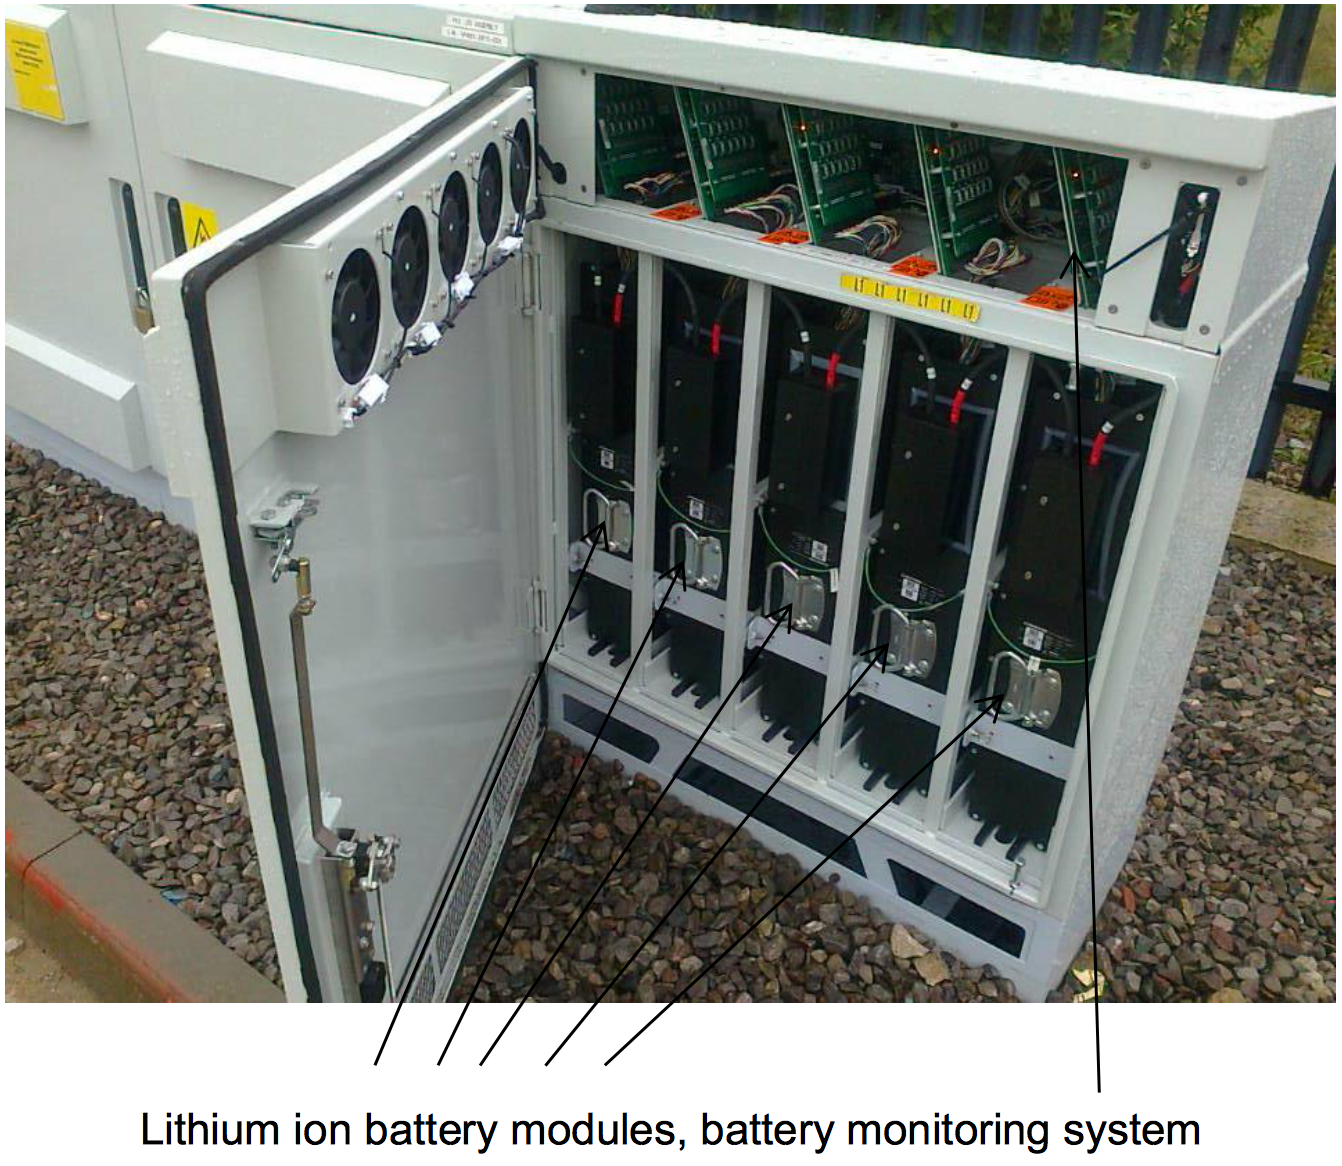
\includegraphics[width=0.415\textwidth]{_literature/fig/esu}
		\label{ch-literature:subfig:esmu-esu}
	}
	\subfloat[]{
		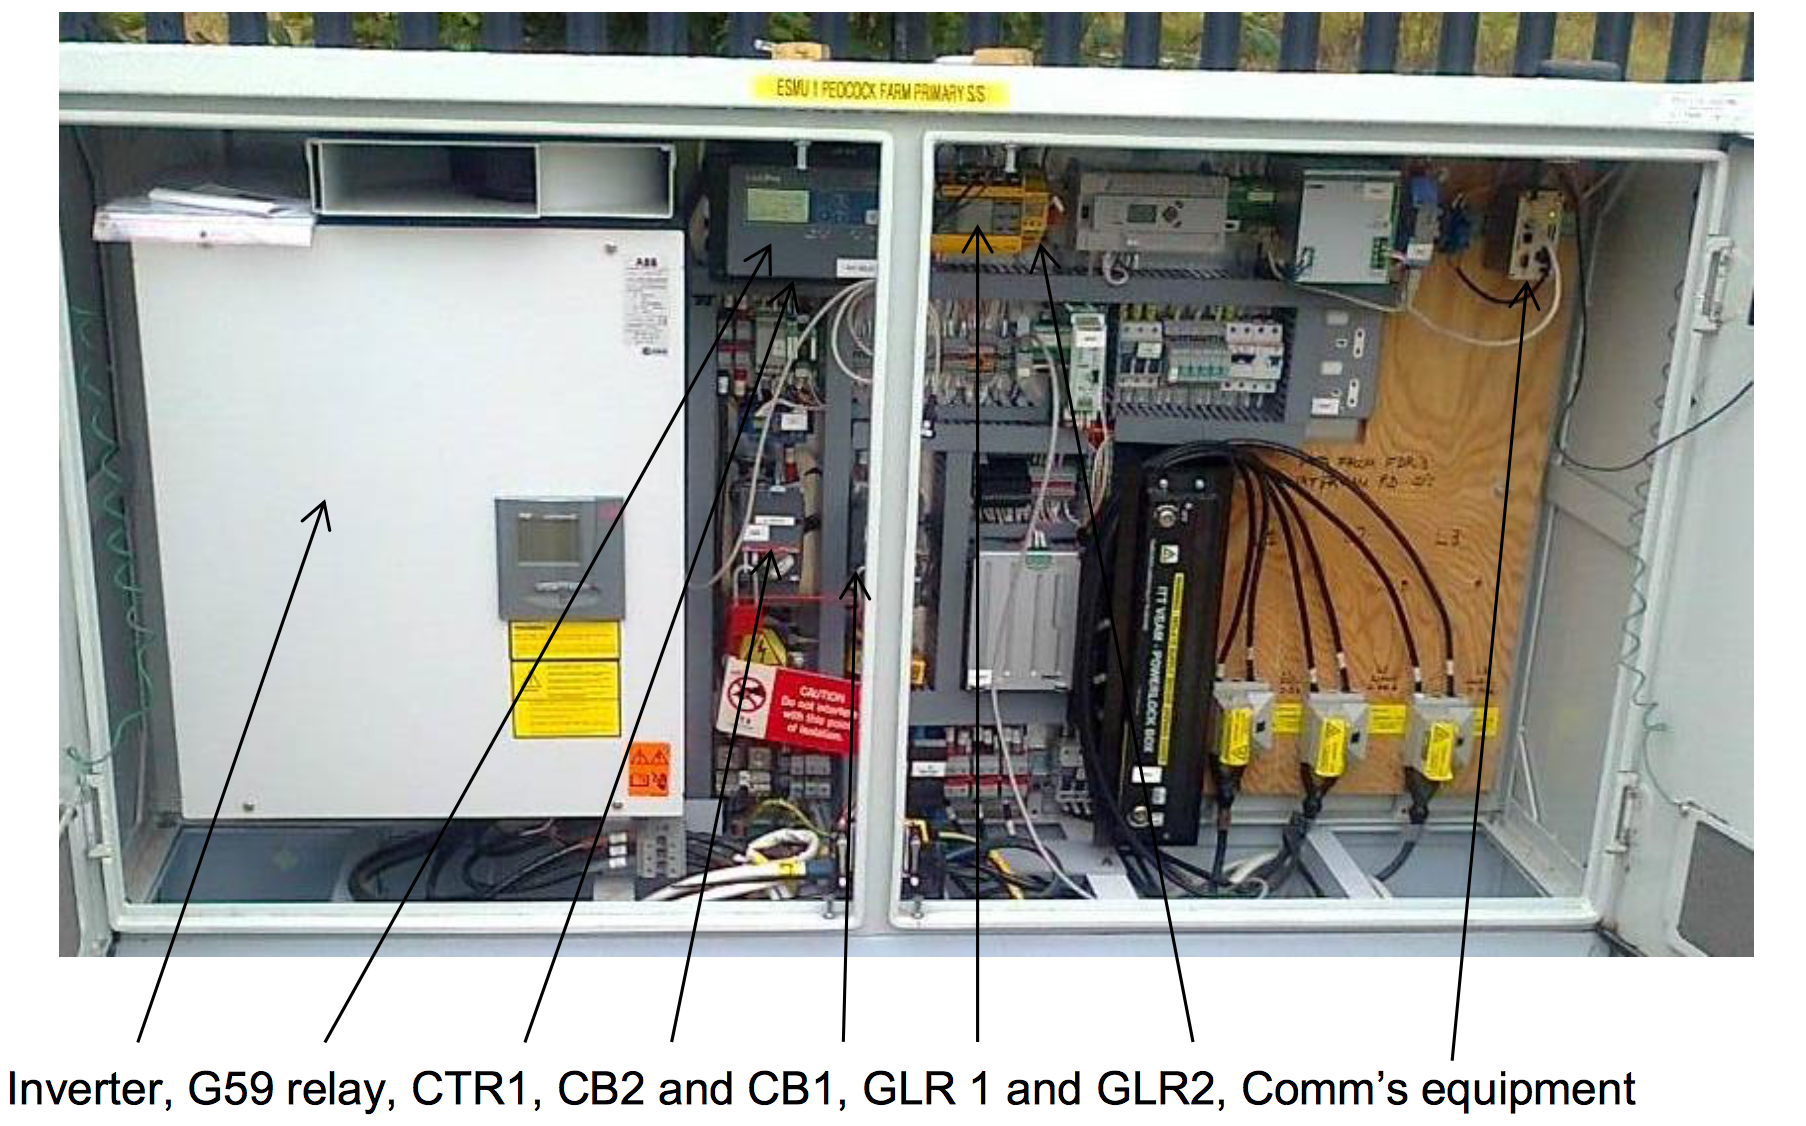
\includegraphics[width=0.585\textwidth]{_literature/fig/peu}
		\label{ch-literature:subfig:esmu-peu}
	}\\
	\subfloat[]{
		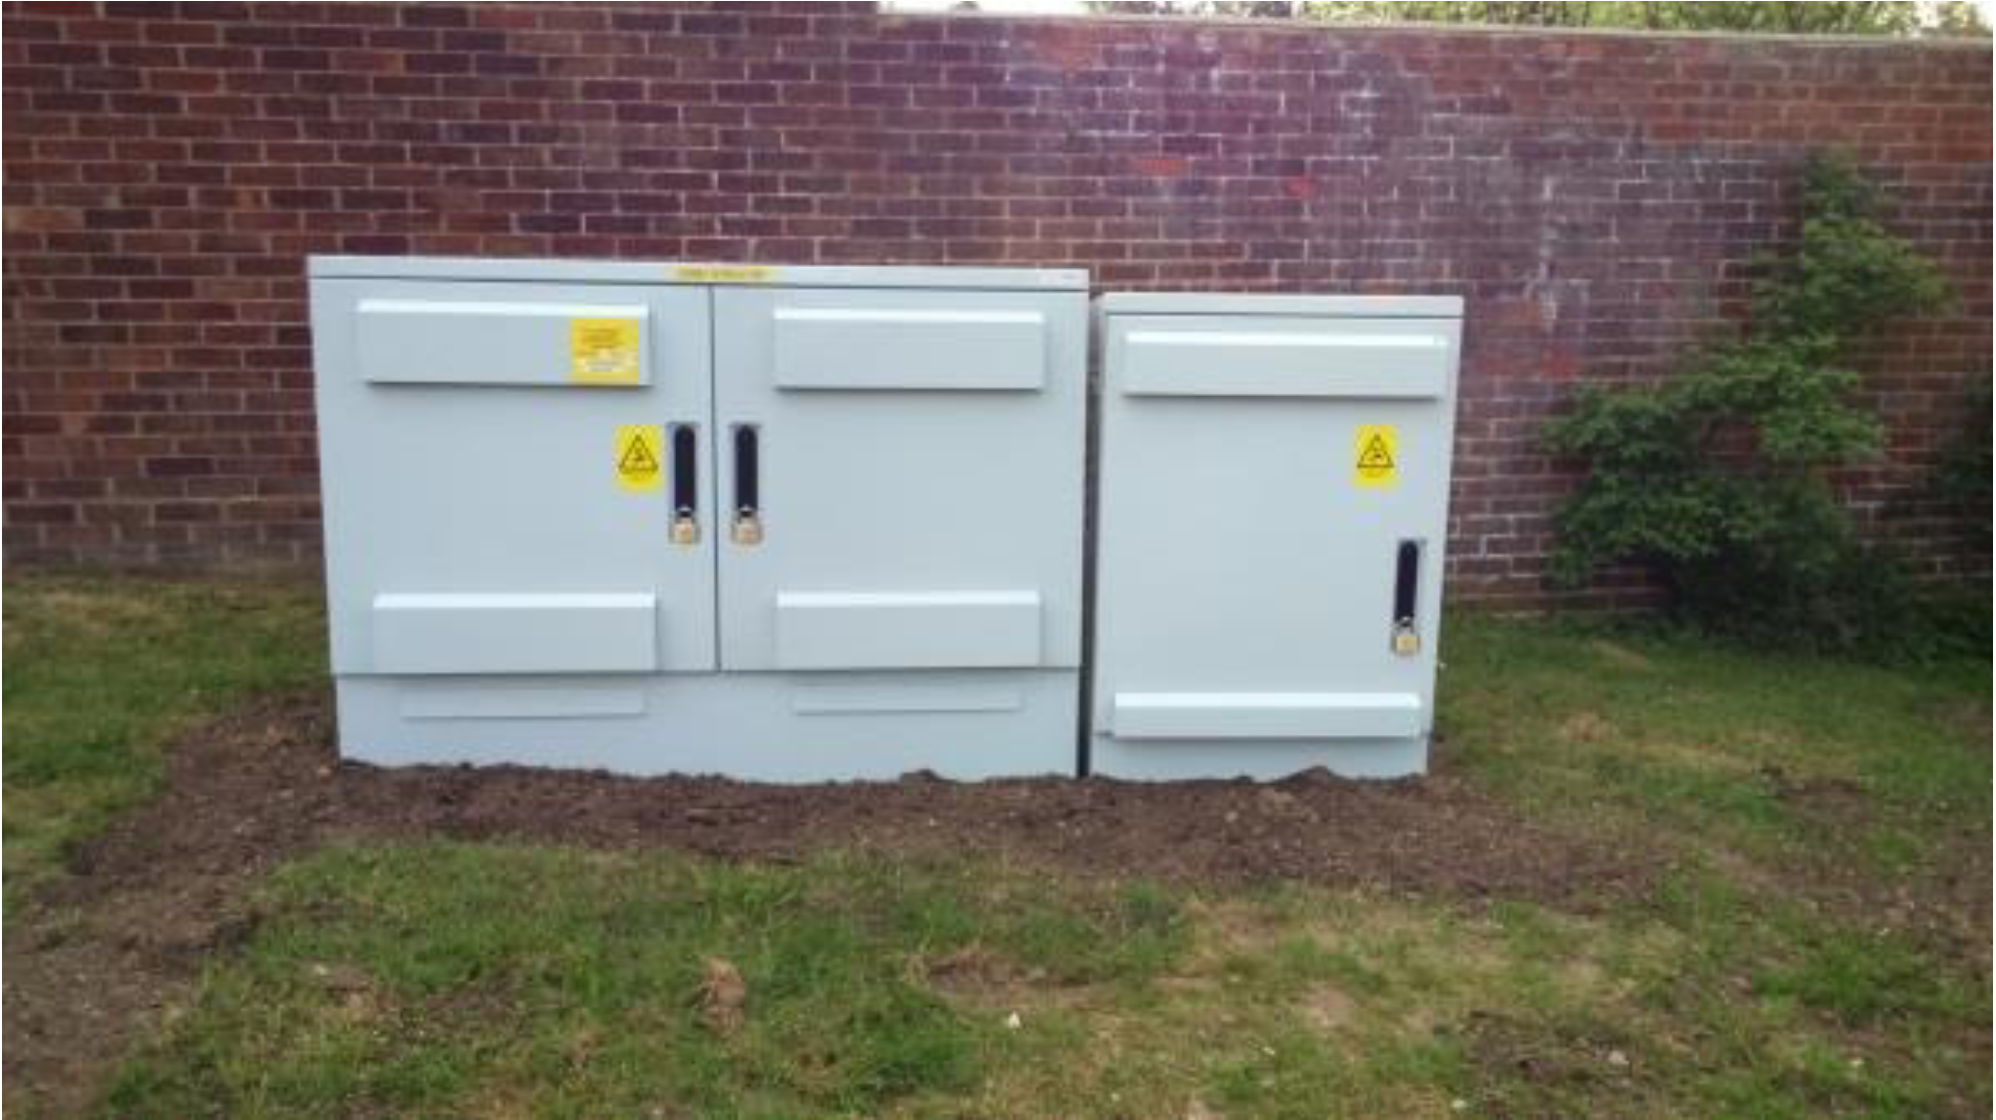
\includegraphics[width=0.7\textwidth]{_literature/fig/esmu-1}
		\label{ch-literature:subfig:esmu-esmu-1}
	}\\
	\subfloat[]{
		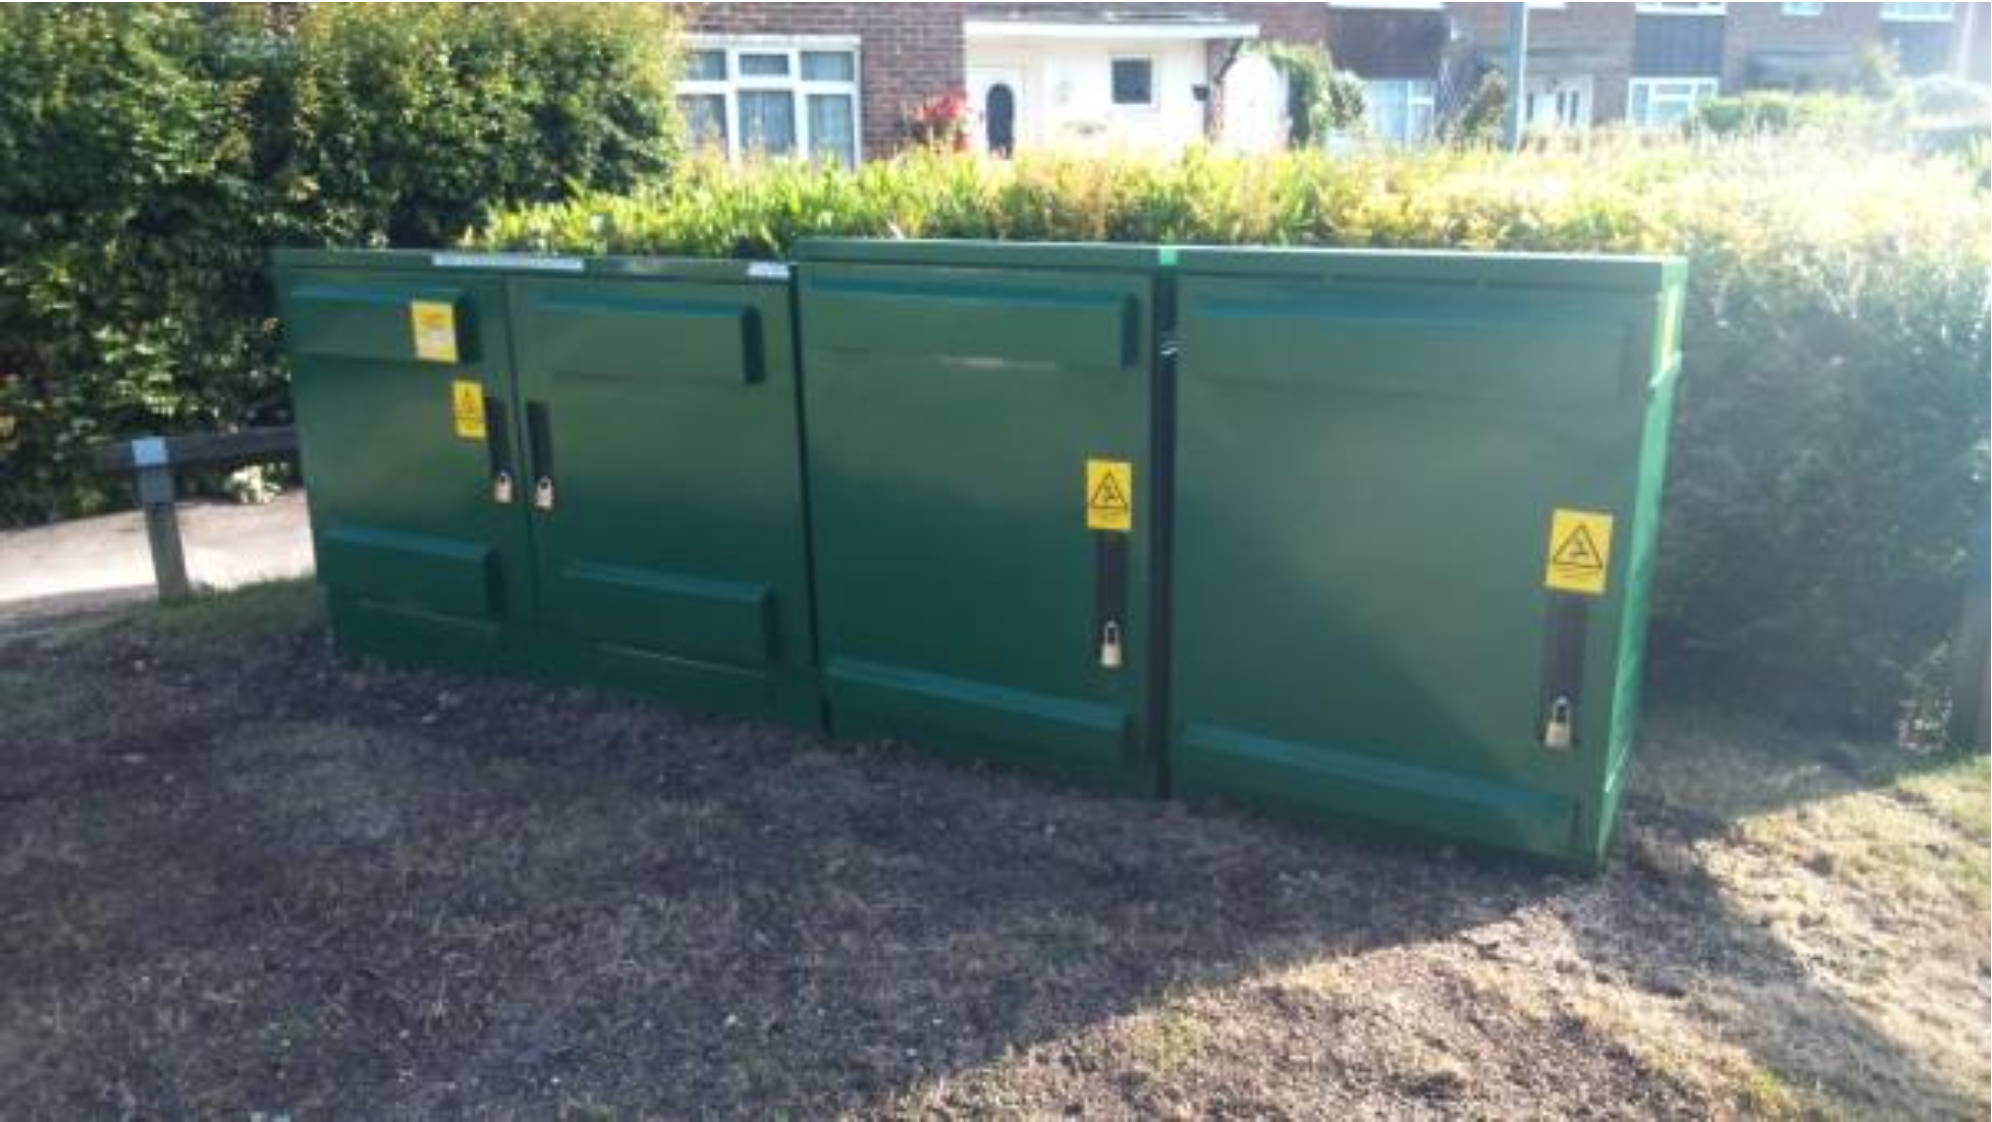
\includegraphics[width=0.7\textwidth]{_literature/fig/esmu-2}
		\label{ch-literature:subfig:esmu-esmu-2}
	}
	\caption{Energy Storage Management Unit overview: (a) 12.5kWh Energy Storage Unit, (b) Power Electronics Unit, (c) deployed 12.5kWh system, (d) deployed 25kWh system - pictures are taken from the NTVV close down report \cite{NTVV9.8a}}
	\label{ch-literature:fig:esmu}
\end{figure}

Aiming to address both voltage and power flow problems, \textit{Scottish and Southern Electricity Networks} (SSEN) became the first UK network operator to trial street-level BESS deployment in the LV network, and they installed 500kWh worth of storage in Bracknell, UK \cite{SSEN2016}.
This capacity was achieved by 25 Energy Storage Management Units (ESMUs), like those pictured in Figure~\ref{ch-literature:fig:esmu}.
Each ESMU had cascadable 12.5kWh Energy Storage Units (ESUs), and the ESUs were connected to the distribution network via a three-phase 36kW Power Electronic Unit (PEU) to both manage the batteries and perform filtering operations.
The aim of this so called \textit{New Thames Valley Vision} (NTVV) project was to understand potential benefits, practicalities and costs of installing street-level BESS.
In the beginning the main problem of finding an optimal deployment location for the ESMUs to achieve their best possible impact on system voltages had to be addressed.
Yunusov et al. and Rowe et al. worked in collaboration with \textit{SSEN}, and they assessed different BESS locations in several networks \cite{Yunusov2016, Rowe2014, Rowe2014a}.
They found that a location 4/7 to 2/3 down the feeder yields the best overall impact on voltage levels and power flow.
However, their findings also show that this location can vary significantly when not focusing on voltage support exclusively; i.e. proximity to the feeding substation was of greater importance when reducing the system's overloads or distribution losses.
Also, the chosen $\text{control system}$ had significant impact on the BESS performance, which is why more emphasis has been put on BESS control instead of locating or constructing BESS.
Therefore, a review of BESS control methods including those that are implemented in the NTVV project are presented in the next section, Section~\ref{ch-literature:sec:control-of-energy-storage}.








